\textbf{Пример пары заданий одного типа, на основе которых создан следующий шаблон. } 

\begin{figure}[h]
		\centering
		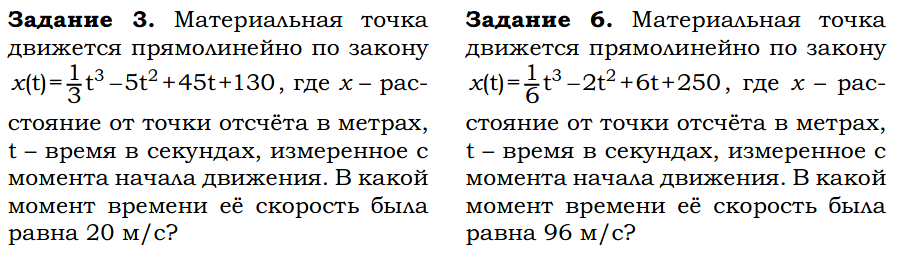
\includegraphics[width=1\linewidth]{VM/Primer.png}
\label{ris:image}
\end{figure}

Первая часть шаблона выглядит следующим образом:

\lstinputlisting{paragrafs/Zadachi/1}

Здесь объявляются переменные таким образом, чтобы генерируемые значения,  максимально соотносились с исходной задачей.

В этой части также используются специальные встроенные функции, такие как:
\\ \texttt{sluchch(a, b)} – функция случайным образом возвращает число из диапазона от \texttt{a} до \texttt{b}. Если функции добавить третье число \texttt{sluchch(a, b, с)}, то она будет возвращать случайно число уже с шагом \texttt{с}.
\\ \texttt{Math.abs(a)} – функция возвращает модуль числа \texttt{a}.
\\ \texttt{function plusmin(member)} – функция принимает аргумент, содержащий в себе пример, наподобие: \texttt{1*a+-b}. И возвращает его упрощённый вариант: \texttt{a-b}.

Вторая часть выглядит следующим образом:

\lstinputlisting{paragrafs/Zadachi/2}

Вторая часть программы делится на несколько составных частей:
\\ условие задачи, записанное после \texttt{text:}
\\ решение, записанное после \texttt{analys:}
\\ ответ, записанный после \texttt{answer}

В этом шаблоне мы вводим переменные, генерирующие случайные значения, которые используем для составления ответа. И на основе ответа мы уже составляем саму задачу и её решение.

В этой части также используются некоторый команды \LaTeX[3], например:
\\ \texttt{\textbackslash frac} – функция выводящая дробь на экран.
\\ \texttt{\textbackslash Rightarrow} – функция выводящая двойную стрелку вправо
\\ \texttt{\textbackslash begin\{cases\}} и \texttt{\textbackslash end\{cases\}} – окружение, выводящая фигурную скобку на экран.

\textbf{ Пример сгенерированных шаблоном задач}

 	\begin{figure}[h]
		\centering
		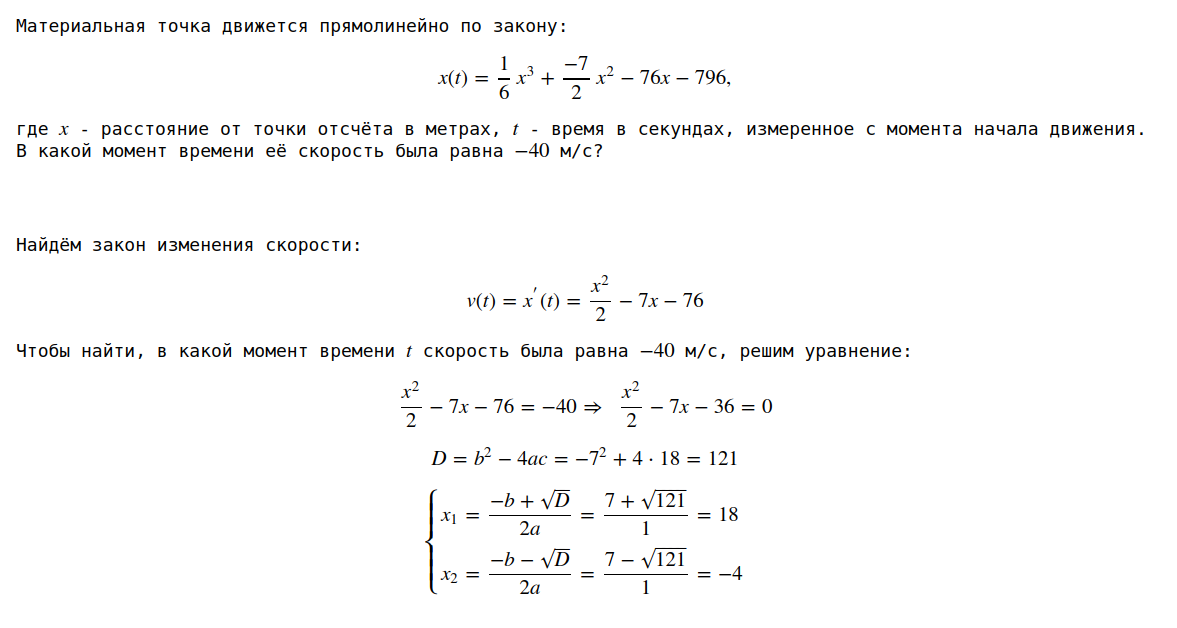
\includegraphics[width=0.85\linewidth]{VM/vch1.png}
		 		\end{figure}
		 	\begin{figure}[h]
		\centering
		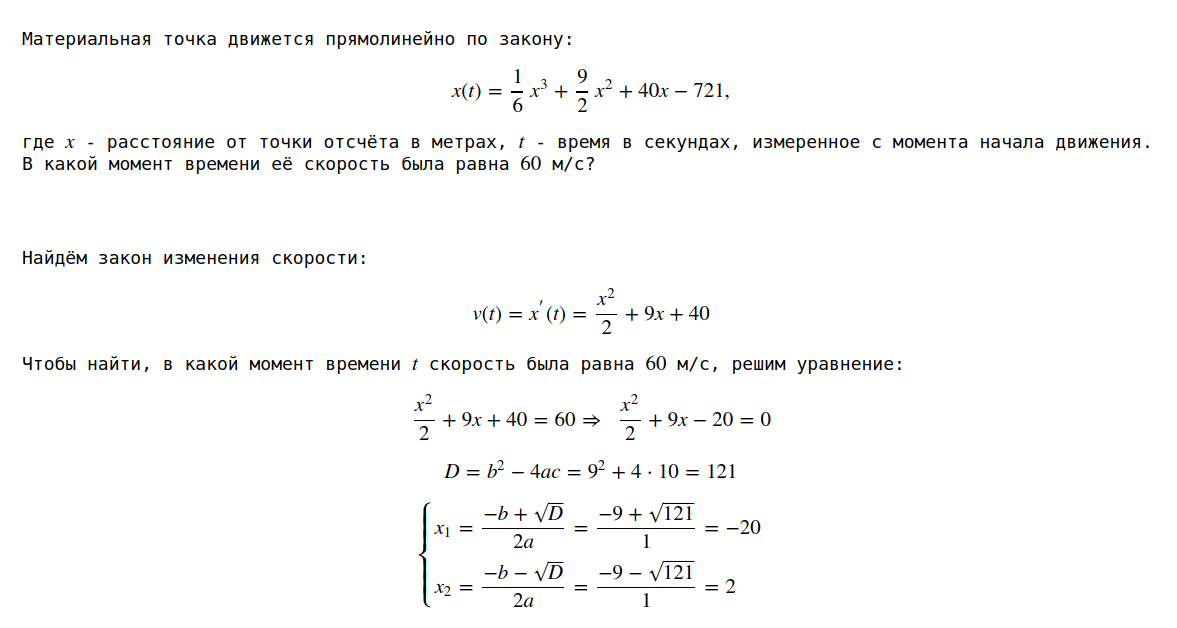
\includegraphics[width=0.85\linewidth]{VM/vch2.png}
	\end{figure}
